\documentclass[a4paper, 12 pt]{article}

\usepackage{graphicx}
\usepackage{bm}

\author{Guillaume Tollini}

\title{TVC Rocket dynamics}

\date{\vfill \today}

\begin{document}

\maketitle

\newpage

\section*{Objective}
\addcontentsline{toc}{section}{\protect\numberline{}Objective}
This document aims at giving all the keys to understand the dynamics of an UAV.

\newpage

\tableofcontents

\newpage


\section{Mathematical model}
\subsection{Reference frames}
\begin{figure}[!h]
\hspace{0 cm}
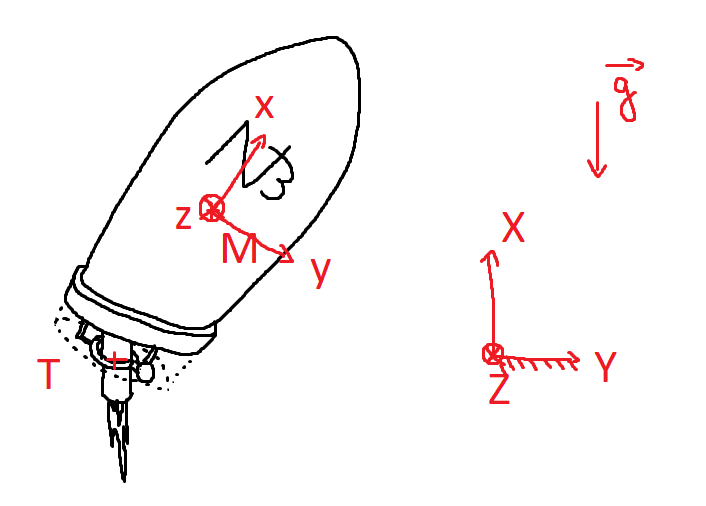
\includegraphics[width=0.9\textwidth]{schema-fusee.png}
\caption{Reference frames}
\end{figure}

$\mathcal{R}_{Earth}$ is the inertial reference frame that is fixed to Earth, it is associated with the vector basis $\bm x\bm y\bm z$. $\mathcal{R}_{AUV}$ is the reference frame that is fixed to the AUV. It is not inertial and associated with the vector basis $\bm X\bm Y\bm Z$.

\begin{figure}[!h]
\begin{tabular}{| l l c c c |}
\hline
\parbox[t]{2.8 cm}{Degree of\newline freedom (DOF)}	& Description	& \parbox[t]{1.6 cm}{Force or \newline moment}	& Velocity	& \parbox[t]{2.3 cm}{Position and \newline Euler angles} \\
\hline \hline
1			& surge direction (x-axis)			& $X$	& u		& $x$ \\
2			& sway direction (y-axis)			& $Y$	& v		& $y$ \\
3			& heave direction (z-axis)			& $Z$	& w		& $z$ \\
4			& roll : rotation about the (x-axis)		& $K$	& p		& $\phi$ \\
5			& pitch : rotation about the (y-axis)		& $M$	& q		& $\theta$ \\
6			& yaw : rotation about the (z-axis)		& $N$	& r		& $\psi$ \\
\hline
\end{tabular}
\caption{Main variables of movement}
\label{variables}
\end{figure}

\subsection{Definition of vectors of interest}
In this document, all vectors and matrices will appear in bold. Vectors defined here after will be used in the mathematical model of tue AUV :

$$\bm\eta = \left[ 
\begin{array}{c}
\bm{\eta}_1	\\
\bm{\eta}_2
\end{array}
\right], \; \bm{\eta}_1 = \left[ 
\begin{array}{c}
x	\\
y	\\
z
\end{array}
\right], \; 
{\bm\eta}_2 = \left[ 
\begin{array}{c}
\phi	\\
\theta	\\
\psi
\end{array}
\right]$$

$$\bm\nu = \left[ 
\begin{array}{c}
\bm{\nu}_1	\\
\bm{\nu}_2
\end{array}
\right], \; \bm{\nu}_1 = \left[ 
\begin{array}{c}
u	\\
v	\\
w
\end{array}
\right], \; 
{\bm\nu}_2 = \left[ 
\begin{array}{c}
p	\\
q	\\
r
\end{array}
\right]$$

$$\bm\tau = \left[ 
\begin{array}{c}
\bm{\tau}_1	\\
\bm{\tau}_2
\end{array}
\right], \; \bm{\tau}_1 = \left[ 
\begin{array}{c}
X	\\
Y	\\
Z
\end{array}
\right], \; 
{\bm\tau}_2 = \left[ 
\begin{array}{c}
K	\\
M	\\
N
\end{array}
\right]$$

\section{Equations of movement}

$$\bm M_{RB}\cdot \bm \dot{\nu} + \bm C_{RB}\cdot \nu = \tau$$

\section{Forces}

The vector $\bm \tau$ of forces and moments can be decomposed into several vectors, each regrouping the actions of different physical origins :

\begin{itemize}
\item $\bm {\tau}_G$ for the action of gravity
\item $\bm {\tau}_D$ for the drag due to the surrounding air
\item $\bm {\tau}_C$ for the actions influenced by the control inputs
\end{itemize}

\subsubsection{Weight}

$\bm W$ is the weight vector of the rocket.
Then $\bm W_{\mathcal{B}} = \bm W|{\bm x\bm y\bm z} = [-m.g \; 0 \; 0]^T$ ($\bm x$ is upwards).
Since $\bm W|{\bm x\bm y\bm z} = \bm J_1\cdot \bm W|_{\mathcal{B}}$, 
then $\bm W|{\bm x\bm y\bm z} = \bm J_1^{-1}\cdot \bm W|_{\mathcal{B}}$.
And because $\bm J_1$ is orthogonal, $\bm J_1^{-1} = \bm J_1^T$. So we have :

$$\begin{array}{l l}
\bm {\tau}_G|_{\mathcal{B}} & = \left[
\begin{array}{c}
\bm J_1^T\cdot(\bm W|_{\mathcal{B}} + \bm B|_{\mathcal{B}})	\\
\bm r_G\times\bm J_1^T\cdot\bm W|_{\mathcal{B}} + \bm r_B\times\bm J_1^T\cdot\bm B|_{\mathcal{B}})
\end{array}
\right]	\\ 
& \\
& = \left[
\begin{array}{c}
\bm J_1^T\cdot(\bm W|_{\mathcal{B}} + \bm B|_{\mathcal{B}})	\\
\bm S(r_G)\cdot\bm J_1^T\cdot\bm W|_{\mathcal{B}} + \bm S(\bm r_B)\cdot\bm J_1^T\cdot\bm B|_{\mathcal{B}}
\end{array}\right]\end{array}$$
\end{array}
\right]$$

\subsection{Drag}


\subsection{Thrust vector control}

Let us call $T$ the norm of the thrust vector (which is the action of thrust on the rocket). We rotate the rocket-fixed reference frame $\bm{xyz}$ of an angle $\alpha_1$ about $\bm y$ and
name the new reference frame $\bm{x'yz'}$. We then rotate this reference frame of an angle $\alpha_2$ about $\bm z'$ and we get the reference frame
$\bm{x''y'z'}$. $\bm x''$ is the vector carrying th thrust vector. $\alpha_1$ and $\alpha_2$ are the two command angles.

We have :

$$\bm{\tau}_C = T \bm x'' = \bm R_Z(\alpha_2) \cdot \bm R_Y(\alpha_1) \cdot \left[\begin{array}{c} T \\ 0 \\ 0 \end{array}\right]$$



\end{document}